\documentclass[8pt]{beamer}
\usepackage[nobglogo]{beamerthemedmi-owled}
\usepackage[utf8x]{inputenc}
\usepackage{default}
\usepackage{url}
\usepackage{verbatim}
\usepackage{graphicx}
\usepackage{mathrsfs}
\usepackage{dl}
\usepackage{mls}

\mode<presentation>
{
  \usetheme{dmi-owled}
  %\usetheme{Warsaw}
  % or ...

  \setbeamercovered{transparent}
  % or whatever (possibly just delete it)
}

\title{Web Reasoning 2015/2016\\
Lezione 2}

\author{Cristiano Longo\\ 
{\small{longo@dmi.unict.it}}}



\date{Universit\`a di Catania}
\newcommand{\urlsingle}[1]{{\small {\center {\url{#1}}}}}
\begin{document}
\maketitle
\setcounter{tocdepth}{1}

\section{URI/IRI}

\begin{frame}
	\frametitle{The Semantic Web Stack}
	L'insieme delle tecnologie impiegate nel Web Semantico
	costituisce il \emph{Semantic Web Stack}.

	\phantom{Tratteremo la gran parte di queste.}

	\begin{figure}
	    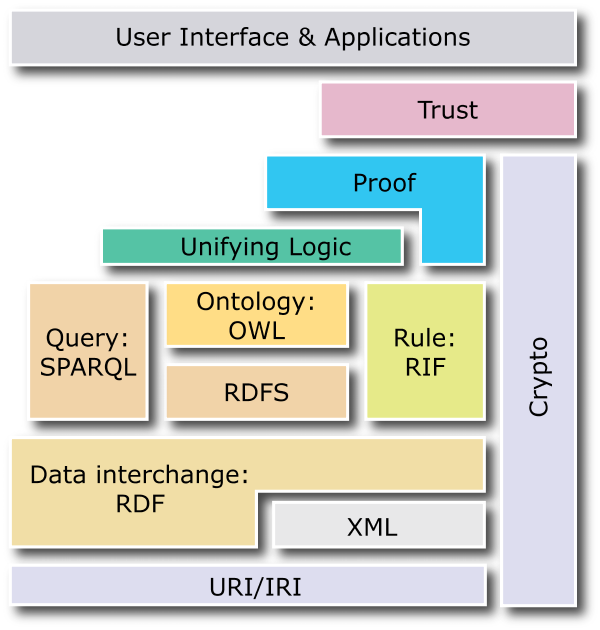
\includegraphics[width=180px]{imgs/Semantic_Web_Stack0.png}
	    \caption{The Semantic Web Stack}
	\end{figure}
\end{frame}

\begin{frame}
	\frametitle{The Semantic Web Stack}
	L'insieme delle tecnologie impiegate nel Web Semantico 
	costituisce il \emph{Semantic Web Stack}.
	
	Tratteremo la gran parte di queste.
	
	\begin{figure}
	    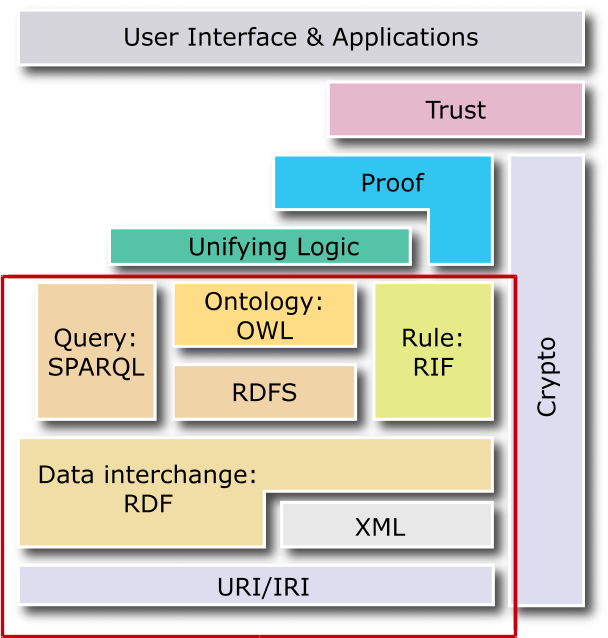
\includegraphics[width=180px]{imgs/Semantic_Web_Stack0all.png}
	    \caption{The Semantic Web Stack} 
	\end{figure}
\end{frame}

\begin{frame}
	\frametitle{URI/IRI}
	
	\begin{itemize}
	  \item \emph{Uniform Resource Identifiers} (URI) - RFC3986
	  \item \emph{Internationalized Resource Identifiers (IRIs)} (IRI) - RFC3987
	\end{itemize}	
	
	Nel Web Semantico le IRI servono ad \emph{indicare} oggetti di qualsiasi
	natura, concreti o astratti.
	
	\begin{figure}
	    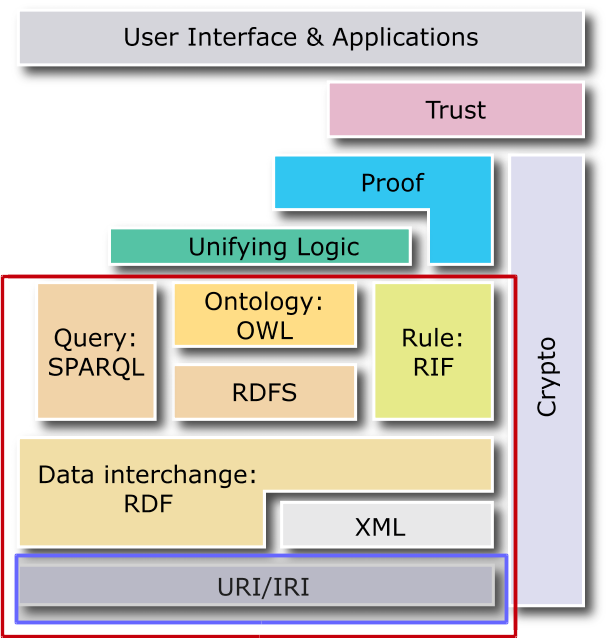
\includegraphics[width=180px]{imgs/Semantic_Web_Stack_uri.png}
	    \caption{The Semantic Web Stack} 
	\end{figure}
\end{frame}

\begin{frame}
	\frametitle{URI - ABNF}
	TODO
\end{frame}

\begin{frame}
	\frametitle{URI - percent encoding}
	TODO
\end{frame}

\begin{frame}[fragile]
	\frametitle{URI - caratteri riservati}
	
	I caratteri riservati solitamente ricoprono la funzione di 
	separatori per delimitare le varie parti della URI.
	
	\begin{verbatim}
 reserved    = gen-delims / sub-delims
 
 gen-delims  = ":" / "/" / "?" / "#" / "[" / "]" / "@"

 sub-delims  = "!" / "$" / "&" / "'" / "(" / ")"
                  / "*" / "+" / "," / ";" / "=" 
                  

                  
	\end{verbatim}
	\vspace{\baselineskip}
	
\uncover<2->{
	Nel caso in cui si abbia la necessit\`a di usare caratteri riservati
	nel corpo di alcune parti della URI e non come separatori, \'e possibile
	farlo applicando il percent-encodind.
	\vspace{\baselineskip}
}

\phantom{
 	I caratteri che possono comparire all'interno delle parti di una URI
 	sono detti \emph{non riservati}. In alre parole, i caratteri non riservati
 	sono tutti i caratteri permessi in una URI ad esclusione di quelli riservati.
}	
\end{frame}

\begin{frame}[fragile]
	\frametitle{URI - caratteri riservati}
	
	I caratteri riservati solitamente ricoprono la funzione di 
	separatori per delimitare le varie parti della URI.
	
	\begin{verbatim}
 reserved    = gen-delims / sub-delims
 
 gen-delims  = ":" / "/" / "?" / "#" / "[" / "]" / "@"

 sub-delims  = "!" / "$" / "&" / "'" / "(" / ")"
                  / "*" / "+" / "," / ";" / "=" 
                  
 unreserved  = ALPHA / DIGIT / "-" / "." / "_" / "~"
                  
	\end{verbatim}
	\vspace{\baselineskip}
	
	Nel caso in cui si abbia la necessit\`a di usare caratteri riservati
	nel corpo di alcune parti della URI e non come separatori, \'e possibile
	farlo applicando il percent-encodind.
	\vspace{\baselineskip}

 	I caratteri che possono comparire all'interno delle parti di una URI
 	sono detti \emph{non riservati}. In alre parole, i caratteri non riservati
 	sono tutti i caratteri permessi in una URI ad esclusione di quelli riservati.	
\end{frame}

\begin{frame}[fragile]
	\frametitle{URI - componenti di una URI}
	
	La sintassi delle URI \`e definita come segue:
	
	\begin{verbatim}
  URI = scheme ":" hier-part [ "?" query ] [ "#" fragment ]

  hier-part   = "//" authority path-abempty
              / path-absolute
              / path-rootless
              / path-empty                  
	\end{verbatim}
	\vspace{\baselineskip}
	
	Riportiamo due esempi di uri.
	\vspace{\baselineskip}

	\begin{figure}
	    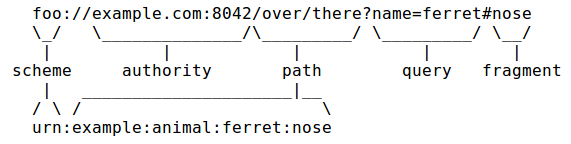
\includegraphics[width=250px]{imgs/uri-pieces.png}
	    \caption{Esempi di URI}
	\end{figure}
	
\end{frame}

\begin{frame}[fragile]
	\frametitle{URI - componenti - schema}
    Ogni URI inizia con uno \emph{schema}. Ogni schema identificana
    ulteriori restrizioni sintattiche nelle URI che vi ricadono.
    Alcuni schemi noti sono \tt{http}, \tt{mail}, \tt{tel}.\footnote{Un elenco
    esaustivo di URI scheme \`e disponibile alla pagina
    \url{http://www.iana.org/assignments/uri-schemes/uri-schemes.xhtml}.}
    \vspace{\baselineskip}
    
    Gli schemi hanno la seguente sintassi
    \begin{verbatim}
  scheme = ALPHA *( ALPHA / DIGIT / "+" / "-" / "." )
    \end{verbatim}    
\end{frame}

% The process for registration of new URI schemes is
%    defined separately by [BCP35].  Advice for designers of new URI
%    schemes can be found in [RFC2718]. 

% Each URI begins with a scheme name, as defined in Section 3.1, that
%    refers to a specification for assigning identifiers within that
%    scheme.  As such, the URI syntax is a federated and extensible naming
%    system wherein each scheme's specification may further restrict the
%    syntax and semantics of identifiers using that scheme.

% URI "resolution" is the process of
%    determining an access mechanism and the appropriate parameters
%    necessary to dereference a URI; this resolution may require several
%    iterations.  To use that access mechanism to perform an action on the
%    URI's resource is to "dereference" the URI.

% A percent-encoding mechanism is used to represent a data octet in a
%    component when that octet's corresponding character is outside the
%    allowed set or is being used as a delimiter of, or within, the
%    component.  A percent-encoded octet is encoded as a character
%    triplet, consisting of the percent character "%" followed by the two
%    hexadecimal digits representing that octet's numeric value.  For
%    example, "%20" is the percent-encoding for the binary octet
%    "00100000" (ABNF: %x20)
\end{document}
